\documentclass[12pt,letterpaper,noanswers]{exam}
\usepackage[usenames,dvipsnames,svgnames,table]{xcolor}
\usepackage[margin=0.9in]{geometry}
\renewcommand{\familydefault}{\sfdefault}
\usepackage{multicol}
\pagestyle{head}
\header{AM 108 Class 02}{Updated \today.}{Phase portraits}
\runningheadrule
\headrule
\usepackage{graphicx} % more modern
\usepackage{amsmath} 
\usepackage{amssymb} 
\usepackage{hyperref}
\usepackage{tcolorbox}

\begin{document}
 \pdfpageheight 11in 
  \pdfpagewidth 8.5in

% Names: \rule{2.5in}{0.5pt}
% \vspace{0.2cm}

% Goals: be exposed to a map.
% Look at long term behavior.

% Pre-work: define "is and element of", "the real numbers", and "maps to"
\begin{itemize}
    \item There is a pre-class video assignment for Class 03 (C03) due on Wednesday September 9th at 1:20pm.  See Canvas for more info.  
    
    \emph{I have added a short flipgrid assignment to this pre-class assignment.  I am adding this because it is harder for me to feel like I am meeting you in our remote setting.}
    \item There is a problem set due Friday September 11th at 5pm ET.  It will be posted to Canvas early tomorrow (or late today).
    
    \emph{Given the circumstances of the semester, all students have access to deadline flexibility on problem sets this semester.  Notify the course staff via a private message on Piazza if you need a short extension, letting us know when you plan to submit the assignment.  You can assume the extension request will be granted even if you don't hear back from us immediately}
    \item Our first skill check will be due by the end of day on Wednesday Sept 9th.  The sample question is below (just before today's in-class problems).  The skill check itself will be very similar (but not identical) to the question below.
\end{itemize}

\hrule
\vspace{0.2cm}




\noindent \textbf{Extra vocabulary:}
\begin{tcolorbox}
\textbf{hyperbolic fixed point} or \textbf{hyperbolic equilibrium point}. For a 1d flow (a first order differential equation that defines a dynamical system) given by $\dot x = f(x)$, a fixed point or equilibrium point, $x^*$, of the dynamical system is called \emph{hyperbolic} if  $\left.\frac{df}{dx}\right\vert_{x^*} \neq 0$.

In contrast, a fixed point is called \textbf{non-hyperbolic} if $f'(x^*) = 0$.

\end{tcolorbox}

Fixed points where linear stability analysis tells us their stability are hyperbolic fixed points.  Fixed points where we have to go beyond the linear stability analysis are non-hyperbolic.
\vfill

\vspace{0.2cm}

\hrule
\vspace{0.2cm}

\noindent \textbf{Solutions to} $\dfrac{dx}{dt} = a x$

When we linearize a 1d flow about a hyperbolic fixed point the resulting system is of the form $\dfrac{dx}{dt} = a x$.

This is a
\begin{itemize}
\itemsep-0.3em
    \item deterministic
    \item continuous
    \item linear
    \item autonomous (the dynamical rule depends does not depend on the current time)
    \item 1d
\end{itemize}
dynamical system.

Solutions are of the form $x(t) = x_0 e^{at}$.

\vspace{3in}

\vspace{0.2cm}

\hrule
\vspace{0.2cm}


\noindent \textbf{Addressing your questions:}

Section 2.2: finding fixed points.
\begin{enumerate}
\itemsep-0.2em
    \item For $\dot x = x - \cos x$, why does the graphical approach involve plotting two functions? 
\end{enumerate}


Section 2.4: linear stability analysis.
\begin{enumerate}
\itemsep-0.2em
    \item In deriving the linearization, why is $\dot \eta = f(x^* + \eta)$?
    \item How is the expression for the linearization derived?
    \item Why can the $\mathcal{O}(\eta^2)$ terms be neglected for $f'(x^*)\neq 0$, but can't be neglected for $f'(x^*) = 0$?
    \item What is useful about knowing the characteristic timescale (set by $f'(x^*)$) in $\dot \eta = f'(x^*)\eta$?
\end{enumerate}

Section 2.5: uniqueness of solutions
\begin{enumerate}
\itemsep-0.2em
    \item Is there anything special that we do when a system has non-unique solutions?
    \item Is non-uniqueness of solutions a problem?
\end{enumerate}

Extra note: 

\eject
space for me to write.

\eject



% \noindent \textbf{Mathematica code}: block 1

% \begin{verbatim}
% f[x_] :=  4 x^2 - 16;
% fixedpoints = Solve[f[x] == 0, x]
% fp1 = x /. fixedpoints[[1]]
% fp2 = x /. fixedpoints[[2]]
% g1[u_] := u (f'[x] /. x -> fp1)
% g2[u_] := u (f'[x] /. x -> fp2)
% \end{verbatim}


% block 2:
% \begin{verbatim}
% distance = 0.2;
% sol1 = NDSolve[{u'[t] == g1[u[t]], u[0] == distance}, u, {t, 0, 1}];
% sol2 = NDSolve[{u'[t] == g2[u[t]], u[0] == distance}, u, {t, 0, 1}];
% sol3 =  NDSolve[{x'[t] == f[x[t]], x[0] == distance + fp1}, 
%   x, {t, 0, 1}];
% sol4 =  NDSolve[{x'[t] == f[x[t]], x[0] == distance + fp2}, 
%   x, {t, 0, 0.5}];
% Plot[{(u[t] /. sol1) + fp1 , (u[t] /. sol2) + fp2 , 
%   (x[t] /. sol3), (x[t] /. sol4)}, 
%   {t, 0, 1}, 
%     PlotRange -> {All, {-3, 6}}, AxesLabel -> {"time", "x(t)"}, 
%     LabelStyle -> Medium]
% \end{verbatim}

\vfill

\vspace{0.2cm}

\hrule
\vspace{0.2cm}
\noindent\textbf{Skill check C03 practice} \emph{The skill check will be posted on Wednesday and we will work on it briefly during class.  You will complete it and upload it to Gradescope on your own.  It will have one questions similar, but not identical, to the question below.}

\begin{questions}
% \question Consider the differential equation $\dot{x} = f(x)$ for $f(x)$ given by the graph below.  Draw a phase portrait for $\dot x = f(x)$ on the blank $x$-axis provided below the graph.  Use the conventional shading scheme to indicate stability type for fixed points (including properly half-shaded for half-stable fixed points).

% 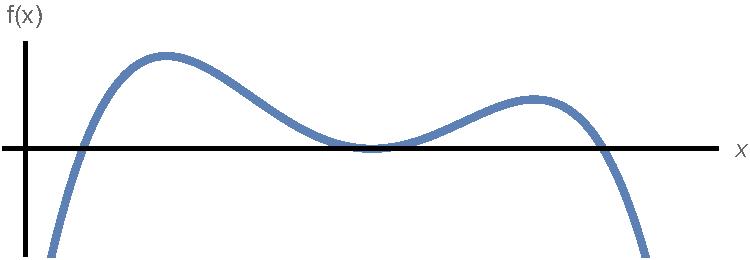
\includegraphics[width=3in]{img/C03prac-2019-09-09phase.pdf}

% 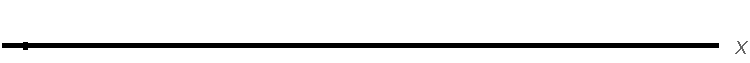
\includegraphics[width=3in]{img/C03prac-2019-09-09axis.pdf}

\question Let $\displaystyle\dot{x} = 4x^2 - 16$.  Use algebraic methods to find the fixed points and to identify their stability.  %Find the fixed points algebraically.  At each fixed point, compute the slope of the vector field.  Use the slope to identify the stability of each fixed point.
\vspace{1in}
\end{questions}

\vspace{0.2cm}

\hrule
\vspace{0.2cm}
\noindent\textbf{Skill check C03 solution}
\begin{enumerate}
\itemsep-0.3em
    \item Set $\dot{x} = 0$ to identify fixed points.
    \item Work out the algebra: $4x^2 - 16 = 0 \Rightarrow x^2 = 4 \Rightarrow x = -2, 2$.  The fixed points are at $x = -2$ and $x = 2$.
    \item Use the slope of $f(x)$ for the stability.  
    \item Find the derivative with respect to $x$: $\dfrac{df}{dx} = 8x$.
    \item Evaluate the slope at the fixed points: $\left.f'(x)\right\vert_{-2} = -16$ and $\left.f'(x)\right\vert_{2} = 16$.
    \item Use the sign of the slope to identify the stability of the fixed point: negative slope means $\dot x > 0$ to the left of the fixed point ($x(t)$ is increasing) and $\dot x < 0$ to the right of the fixed point ($x(t)$ is decreasing).  $x = -2$ is a stable fixed point.  $x = 2$ is an unstable fixed point.
\end{enumerate}
\vspace{0.2cm}

\hrule
\vspace{0.2cm}


\noindent\textbf{Teams}

You have been pre-assigned to a breakout room and team.  There is extra overhead to meeting a group remotely, so we will stay in the same teams for a few class meetings.

\begin{multicols}{2}
1. 
\end{multicols}

\noindent \textbf{Teams 7 and 8}: Post screenshots of your work to the course Google Drive today.  Include words, labels, and other short notes that might make those solutions useful to you or your classmates.  Find the link in Canvas (or here: \url{https://drive.google.com/drive/u/0/folders/1GcpwvKHD4tMecpFQ4lNxN_r5Ylj7YHbd})
\vspace{0.2cm}

\hrule
\vspace{0.2cm}
\eject

\noindent\textbf{Team activity}

\begin{questions}
\question (Plotting a function by hand). The hyperbolic tangent function, $\tanh x = \frac{\sinh x}{\cosh x}$ where $\sinh x = \frac{1}{2}\left(e^{x}-e^{-x}\right)$ and $\cosh x = \frac{1}{2}\left(e^{x}+e^{-x}\right)$, so $\tanh x = \frac{e^x-e^{-x}}{e^x+e^-x}$.

Sketch an approximate plot of $\tanh x$.  Do not use a calculator or other plotting software.

\emph{One way to do this: look at the behavior of the function as $x \rightarrow -\infty$, as $x\rightarrow \infty$, and for $x$ near $0$.  Use the correct slope at $x=0$ and connect up the pieces of the function smoothly.}

Remember axis labels on your plot!  You won't be able to put scale markings on the $x$ axis, but should be able to add them to the vertical axis.

\noindent \textbf{Teams 5 and 6}: Post a written description of your work on this problem in the \#classactivities channel. 


\question
% \begin{tcolorbox}
% Learning aim (procedural): Given a differential equation (a first order dynamical system), students will be asked to run the following procedure and to identify the possible long term behaviors of solutions to the system.
% \end{tcolorbox}

For each of the following, 
\begin{itemize}
\item find the fixed points ({\it{algebraically or graphically, whichever is easier}}), 
\item sketch the phase portrait on the real line
\item classify the stability of the fixed points, 
\item and sketch
approximate time series of $x(t)$ (solutions to the differential equations) for different initial conditions.
\end{itemize}

\noindent \textbf{Teams 3 and 4}: Post a written description of your work on this problem in the \#classactivities channel. 

\begin{parts}

\part $\displaystyle\dot{x} = x - \cos x$. % 
\part $\displaystyle\dot{x} = x/2 - \tanh x$.
\part $\displaystyle\dot{x} = \tanh x - x/2$.
% \part $\dot{x} = x - x^3$.
\end{parts}




\question 

(Strogatz 2.2.10): For each of the following, find an equation $\dot{x} = f(x)$ with the
stated properties, or if there are no examples, explain why not (assume $f(x)$ is smooth).
\begin{parts}
\part Every real number is a fixed point.
\part Every integer is a fixed point and there are no other fixed points.
\part There are precisely three fixed points, and all of them are stable.
\part There are no fixed points.
% \part There are precisely $100$ fixed points.
\end{parts}

\noindent \textbf{Teams 1 and 2}: Post a written description of your work on this problem in the \#classactivities channel. 

\end{questions}


\hrule
\vspace{0.2cm}

\eject


\eject

Suggested extra practice:

\begin{questions}
\question 
\begin{tcolorbox}
Learning aim (procedural): Given a differential equation (a first order dynamical system), students will be asked to identify the possible long term behaviors of solutions to the system using algebraic methods.
\end{tcolorbox}

For the following differential equations, find the fixed points and classify their stability using linear stability analysis (an algebraic method).  If linear stability analysis does not allow you to classify the point, then use a graphical argument.
\begin{parts}
\part  Let $\dot{x} = x(3-x)(1-x)$.   (See Strogatz 2.4.2)
\part Let $\dot{x} = 1- e^{-x^2}$  (Strogatz 2.4.5)
\part  Let $\dot{x} = r x - x^3$ where the parameter $r$ satisfies either $r<0$, $r = 0$, or $r>0$.  Discuss all three cases.  (Strogatz 2.4.7)
\end{parts}



\question


\begin{tcolorbox}
Learning aim (factual, procedural): 


 Given a differential equation (a first order dynamical system), students will be asked to distinguish between parameters and variables.  Students will be asked to define the term \emph{bifurcation diagram}. 
    
    Students will be asked to construct bifurcation diagrams.
\end{tcolorbox}

Let $\dot{x} = r + x^2$.  For $r = -2, -1/4, 0, 1$, find the fixed points and classify their stability ({\it{do this graphically, by plotting $f(x)$ vs $x$, not algebraically}}).  Now, finding the fixed points algebraically as a function of $r$, plot them in the $rx$-plane (so $r$ is along the horizontal axis and the location of the fixed points is along the vertical).  This is a {\it{bifurcation diagram}}, showing the location of fixed points as a parameter changes in the system.  In a bifurcation diagram, stable fixed points are denoted with a solid line while unstable fixed points are denoted with a dashed line.

%\hrule

\question 
\begin{tcolorbox}
Learning aim (procedural, factual): 

Students will be asked to show a particular function is a solution to a differential equation.  

Students will be asked to reason from definitions.
\end{tcolorbox}

(Strogatz 2.6.1) A simple harmonic oscillator, defined by $\displaystyle\ddot{x} = -\frac{k}{m} x$, has a solution $x(t) = A\sin \omega t + B\cos \omega t$ that oscillates on the $x$-axis.
\begin{parts}
\part Plug this expression for $x(t)$ into the differential
equation to show that it is a solution for some $\omega$ and find that $\omega$.  
\item What happens to $A$ and $B$?
\item We learned that oscillations are not possible in a one-dimensional system.  This system is
showing oscillations.  Reconcile those two facts.
\end{parts}

\end{questions}

% \newpage
%  \hfill {\bf \large AM108 1:00pm.  Class 02}
 
%  Extra problems:
% \begin{questions}

% %{\color{blue} Many teams had enough time to get to this point.}

% \item Compare the populations models \[\dot{N} = N(1-N/K)\] (logistic) and 
% \[\dot{N} = N(1-N/K)(N/A-1)\] (strong Allee effect) where $0<A<K$.  
% \begin{parts}
% \item Based on the differential equation, what is the Allee effect?
% \item Try to imagine a scenario where it is relevant (it was initially described in experiments on small fish).
% \item Consider solutions, $N(t)$, to both equations.  
% How, if at all, do solutions between the two equations differ qualitatively?
% \item The term {\it{basin of attraction}} refers to the set of initial conditions that approach a
% particular fixed point.  What is the basin of attraction of the extinction fixed point, $N^*=0$, for each
% equation?
% \end{parts}

% %\hrule

% \item (Strogatz 3.2.3)  Let $\dot{x} = x - r x (1-x)$.  Sketch each of the qualitatively
% different vector fields that occurs as $r$ is varied.  Sketch the bifurcation diagram of fixed points vs $r$
% in the $rx$-plane.
% Use solid and dashed lines to indicate the stability of the fixed points in your diagram.
% \end{questions}
\end{document}

\end{document}